% Options for packages loaded elsewhere
\PassOptionsToPackage{unicode}{hyperref}
\PassOptionsToPackage{hyphens}{url}
\PassOptionsToPackage{dvipsnames,svgnames,x11names}{xcolor}
%
\documentclass[
  12,
]{article}
\usepackage{amsmath,amssymb}
\usepackage{lmodern}
\usepackage{setspace}
\usepackage{iftex}
\ifPDFTeX
  \usepackage[T1]{fontenc}
  \usepackage[utf8]{inputenc}
  \usepackage{textcomp} % provide euro and other symbols
\else % if luatex or xetex
  \usepackage{unicode-math}
  \defaultfontfeatures{Scale=MatchLowercase}
  \defaultfontfeatures[\rmfamily]{Ligatures=TeX,Scale=1}
\fi
% Use upquote if available, for straight quotes in verbatim environments
\IfFileExists{upquote.sty}{\usepackage{upquote}}{}
\IfFileExists{microtype.sty}{% use microtype if available
  \usepackage[]{microtype}
  \UseMicrotypeSet[protrusion]{basicmath} % disable protrusion for tt fonts
}{}
\usepackage{xcolor}
\usepackage{longtable,booktabs,array}
\usepackage{calc} % for calculating minipage widths
% Correct order of tables after \paragraph or \subparagraph
\usepackage{etoolbox}
\makeatletter
\patchcmd\longtable{\par}{\if@noskipsec\mbox{}\fi\par}{}{}
\makeatother
% Allow footnotes in longtable head/foot
\IfFileExists{footnotehyper.sty}{\usepackage{footnotehyper}}{\usepackage{footnote}}
\makesavenoteenv{longtable}
\usepackage{graphicx}
\makeatletter
\def\maxwidth{\ifdim\Gin@nat@width>\linewidth\linewidth\else\Gin@nat@width\fi}
\def\maxheight{\ifdim\Gin@nat@height>\textheight\textheight\else\Gin@nat@height\fi}
\makeatother
% Scale images if necessary, so that they will not overflow the page
% margins by default, and it is still possible to overwrite the defaults
% using explicit options in \includegraphics[width, height, ...]{}
\setkeys{Gin}{width=\maxwidth,height=\maxheight,keepaspectratio}
% Set default figure placement to htbp
\makeatletter
\def\fps@figure{htbp}
\makeatother
\setlength{\emergencystretch}{3em} % prevent overfull lines
\providecommand{\tightlist}{%
  \setlength{\itemsep}{0pt}\setlength{\parskip}{0pt}}
\setcounter{secnumdepth}{5}
\usepackage{hyperref}
\hypersetup{
    colorlinks,
    linkcolor={blue!100!black},
    citecolor={blue!100!black},
    urlcolor={blue!100!black}
}
\usepackage{apacite}
\usepackage[round]{natbib} 
\usepackage{graphicx}
% \usepackage{float}
% \usepackage{caption}
\usepackage[toc,page]{appendix}
\usepackage{booktabs,caption}
% \usepackage[flushleft]{threeparttable}
% \usepackage{tabularx}
\usepackage{amsfonts}
\usepackage{amsmath}
\usepackage{xcolor}
\usepackage{scrextend}
\deffootnote[2em]{2em}{1em}{\textsuperscript{\thefootnotemark}\,}
\newcolumntype{Y}{>{\centering\arraybackslash}X}
\usepackage[a4paper]{geometry}
\usepackage{caption}
\usepackage[bottom,flushmargin,hang,multiple]{footmisc}
\usepackage{pdflscape}
\usepackage[paper=portrait,pagesize]{typearea}
\usepackage{rotating}
\usepackage{fullpage}
\usepackage{tabu}
\usepackage{fontspec}
\usepackage{multirow}
\usepackage{multicol}
\usepackage{colortbl}
\usepackage{hhline}
\usepackage{longtable}
\usepackage{float}
\usepackage{wrapfig}
\usepackage{array}
\usepackage{hyperref}
\ifLuaTeX
  \usepackage{selnolig}  % disable illegal ligatures
\fi
\usepackage[round]{natbib}
\bibliographystyle{apalike}
\IfFileExists{bookmark.sty}{\usepackage{bookmark}}{\usepackage{hyperref}}
\IfFileExists{xurl.sty}{\usepackage{xurl}}{} % add URL line breaks if available
\urlstyle{same} % disable monospaced font for URLs
\hypersetup{
  colorlinks=true,
  linkcolor={blue!000!black},
  filecolor={Maroon},
  citecolor={blue!000!black},
  urlcolor={blue!000!black},
  pdfcreator={LaTeX via pandoc}}

\author{}
\date{\vspace{-2.5em}}

\begin{document}


\title{1929 Herding}


\author { Xolani Sibande\footnote{Department of Economics, University of Pretoria, Pretoria, South Africa; Email: xolaniss@gmail.com.} \,\, 
Rangan Gupta\footnote{Corresponding Author. Department of Economics, University of Pretoria, Pretoria, South Africa; Email: rangan.gupta@up.ac.za.} \,\,
Riza Demirer\footnote{Department of Economics and Finance, Southern Illinois University Edwardsville, Edwardsville, IL 62026-1102, USA}}
\date{\today}
\maketitle

\begin{abstract}


\end{abstract}

\noindent\textbf{Keywords}:   \\
\textbf{JEL Codes}: 
\newpage

\setstretch{1.5}
\hypertarget{introduction}{%
\section{Introduction}\label{introduction}}

\hypertarget{methodology}{%
\section{Methodology}\label{methodology}}

\citet{sim2015oil}

\hypertarget{data}{%
\section{Data}\label{data}}

\newpage

\hypertarget{empirical-results}{%
\section{Empirical Results}\label{empirical-results}}

\providecommand{\docline}[3]{\noalign{\global\setlength{\arrayrulewidth}{#1}}\arrayrulecolor[HTML]{#2}\cline{#3}}

\setlength{\tabcolsep}{0pt}

\renewcommand*{\arraystretch}{1.5}

\begin{longtable}[l]{|p{3.19in}|p{2.77in}}

\caption{\textcolor[HTML]{000000}{\fontsize{8}{10}\selectfont{\global\setmainfont{Helvetica}{General\ heding}}}}\label{tab:gen}\\

\hhline{>{\arrayrulecolor[HTML]{000000}\global\arrayrulewidth=1pt}->{\arrayrulecolor[HTML]{000000}\global\arrayrulewidth=1pt}-}

\multicolumn{1}{!{\color[HTML]{000000}\vrule width 0pt}>{\raggedright}p{\dimexpr 3.19in+0\tabcolsep+0\arrayrulewidth}}{\textcolor[HTML]{000000}{\fontsize{8}{16}\selectfont{\global\setmainfont{Times New Roman}{\ }}}} & \multicolumn{1}{!{\color[HTML]{000000}\vrule width 0pt}>{\raggedright}p{\dimexpr 2.77in+0\tabcolsep+0\arrayrulewidth}!{\color[HTML]{000000}\vrule width 0pt}}{\textcolor[HTML]{000000}{\fontsize{8}{16}\selectfont{\global\setmainfont{Times New Roman}{OLS}}}} \\

\hhline{>{\arrayrulecolor[HTML]{000000}\global\arrayrulewidth=1pt}->{\arrayrulecolor[HTML]{000000}\global\arrayrulewidth=1pt}-}\endhead



\multicolumn{2}{!{\color[HTML]{FFFFFF}\vrule width 0pt}>{\raggedright}p{\dimexpr 5.95in+2\tabcolsep+1\arrayrulewidth}!{\color[HTML]{FFFFFF}\vrule width 0pt}}{\textcolor[HTML]{000000}{\fontsize{8}{16}\selectfont{\global\setmainfont{Times New Roman}{+\ p\ <\ 0.1,\ *\ p\ <\ 0.05,\ **\ p\ <\ 0.01,\ ***\ p\ <\ 0.001}}}} \\

\hhline{>{\arrayrulecolor[HTML]{000000}\global\arrayrulewidth=1pt}->{\arrayrulecolor[HTML]{000000}\global\arrayrulewidth=1pt}-}\endfoot



\multicolumn{1}{!{\color[HTML]{000000}\vrule width 0pt}>{\raggedright}p{\dimexpr 3.19in+0\tabcolsep+0\arrayrulewidth}}{\textcolor[HTML]{000000}{\fontsize{8}{16}\selectfont{\global\setmainfont{Times New Roman}{$\gamma_0$}}}} & \multicolumn{1}{!{\color[HTML]{000000}\vrule width 0pt}>{\raggedright}p{\dimexpr 2.77in+0\tabcolsep+0\arrayrulewidth}!{\color[HTML]{000000}\vrule width 0pt}}{\textcolor[HTML]{000000}{\fontsize{8}{16}\selectfont{\global\setmainfont{Times New Roman}{0.0013***}}}} \\





\multicolumn{1}{!{\color[HTML]{000000}\vrule width 0pt}>{\raggedright}p{\dimexpr 3.19in+0\tabcolsep+0\arrayrulewidth}}{\textcolor[HTML]{000000}{\fontsize{8}{16}\selectfont{\global\setmainfont{Times New Roman}{$\gamma_1 $}}}} & \multicolumn{1}{!{\color[HTML]{000000}\vrule width 0pt}>{\raggedright}p{\dimexpr 2.77in+0\tabcolsep+0\arrayrulewidth}!{\color[HTML]{000000}\vrule width 0pt}}{\textcolor[HTML]{000000}{\fontsize{8}{16}\selectfont{\global\setmainfont{Times New Roman}{0.0013***}}}} \\





\multicolumn{1}{!{\color[HTML]{000000}\vrule width 0pt}>{\raggedright}p{\dimexpr 3.19in+0\tabcolsep+0\arrayrulewidth}}{\textcolor[HTML]{000000}{\fontsize{8}{16}\selectfont{\global\setmainfont{Times New Roman}{$\gamma_2$}}}} & \multicolumn{1}{!{\color[HTML]{000000}\vrule width 0pt}>{\raggedright}p{\dimexpr 2.77in+0\tabcolsep+0\arrayrulewidth}!{\color[HTML]{000000}\vrule width 0pt}}{\textcolor[HTML]{000000}{\fontsize{8}{16}\selectfont{\global\setmainfont{Times New Roman}{0.0000*}}}} \\

\hhline{>{\arrayrulecolor[HTML]{000000}\global\arrayrulewidth=1pt}->{\arrayrulecolor[HTML]{000000}\global\arrayrulewidth=1pt}-}



\multicolumn{1}{!{\color[HTML]{000000}\vrule width 0pt}>{\raggedright}p{\dimexpr 3.19in+0\tabcolsep+0\arrayrulewidth}}{\textcolor[HTML]{000000}{\fontsize{8}{16}\selectfont{\global\setmainfont{Times New Roman}{Num.Obs.}}}} & \multicolumn{1}{!{\color[HTML]{000000}\vrule width 0pt}>{\raggedright}p{\dimexpr 2.77in+0\tabcolsep+0\arrayrulewidth}!{\color[HTML]{000000}\vrule width 0pt}}{\textcolor[HTML]{000000}{\fontsize{8}{16}\selectfont{\global\setmainfont{Times New Roman}{25292}}}} \\





\multicolumn{1}{!{\color[HTML]{000000}\vrule width 0pt}>{\raggedright}p{\dimexpr 3.19in+0\tabcolsep+0\arrayrulewidth}}{\textcolor[HTML]{000000}{\fontsize{8}{16}\selectfont{\global\setmainfont{Times New Roman}{R2}}}} & \multicolumn{1}{!{\color[HTML]{000000}\vrule width 0pt}>{\raggedright}p{\dimexpr 2.77in+0\tabcolsep+0\arrayrulewidth}!{\color[HTML]{000000}\vrule width 0pt}}{\textcolor[HTML]{000000}{\fontsize{8}{16}\selectfont{\global\setmainfont{Times New Roman}{0.613}}}} \\





\multicolumn{1}{!{\color[HTML]{000000}\vrule width 0pt}>{\raggedright}p{\dimexpr 3.19in+0\tabcolsep+0\arrayrulewidth}}{\textcolor[HTML]{000000}{\fontsize{8}{16}\selectfont{\global\setmainfont{Times New Roman}{R2\ Adj.}}}} & \multicolumn{1}{!{\color[HTML]{000000}\vrule width 0pt}>{\raggedright}p{\dimexpr 2.77in+0\tabcolsep+0\arrayrulewidth}!{\color[HTML]{000000}\vrule width 0pt}}{\textcolor[HTML]{000000}{\fontsize{8}{16}\selectfont{\global\setmainfont{Times New Roman}{0.613}}}} \\





\multicolumn{1}{!{\color[HTML]{000000}\vrule width 0pt}>{\raggedright}p{\dimexpr 3.19in+0\tabcolsep+0\arrayrulewidth}}{\textcolor[HTML]{000000}{\fontsize{8}{16}\selectfont{\global\setmainfont{Times New Roman}{Std.Errors}}}} & \multicolumn{1}{!{\color[HTML]{000000}\vrule width 0pt}>{\raggedright}p{\dimexpr 2.77in+0\tabcolsep+0\arrayrulewidth}!{\color[HTML]{000000}\vrule width 0pt}}{\textcolor[HTML]{000000}{\fontsize{8}{16}\selectfont{\global\setmainfont{Times New Roman}{Newey-West}}}} \\

\hhline{>{\arrayrulecolor[HTML]{000000}\global\arrayrulewidth=1pt}->{\arrayrulecolor[HTML]{000000}\global\arrayrulewidth=1pt}-}



\end{longtable}

\newpage

\begin{figure}
\centering
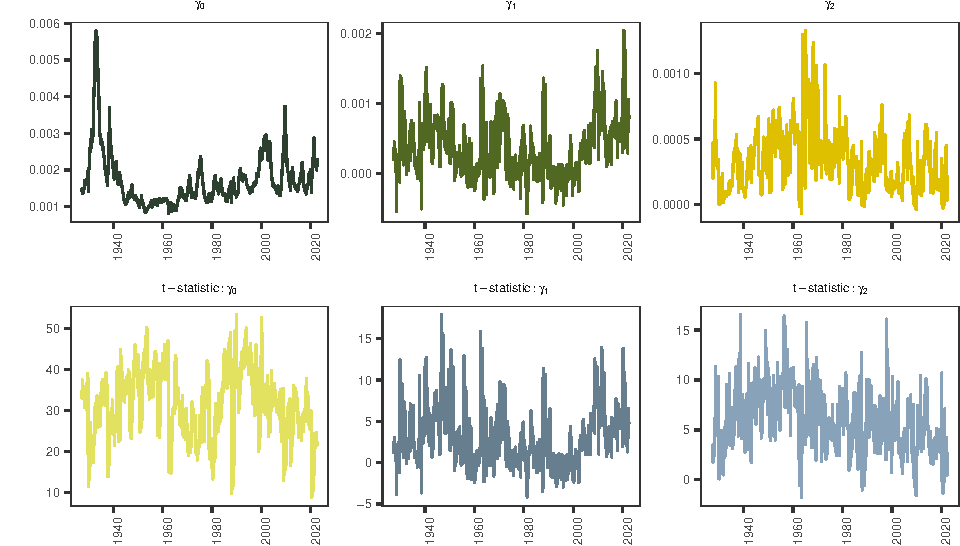
\includegraphics{1929_herding_files/figure-latex/rol-1.pdf}
\caption{\label{fig:rol}CSAD rolling}
\end{figure}

\newpage

\hypertarget{conclusion}{%
\section{Conclusion}\label{conclusion}}

\newpage

\renewcommand\refname{References}
  \bibliography{references.bib}

\newpage
\begin{appendices}


\section{Data}



\section{Descriptive statistics}





\section{Statistical tests}

\end{appendices}

\end{document}
